\documentclass[a4paper, 11pt]{article}

\usepackage{natbib}
\usepackage{graphicx}
\usepackage{epstopdf}
\usepackage[margin = 1 in]{geometry}
\usepackage{multirow}
\usepackage{url}
\usepackage{float}
\usepackage{titlesec}
\usepackage{sectsty}
\usepackage{subcaption}
\usepackage{mwe}

\title{Report Draft}
\author{Weijiang Lin}

\begin{document}

\section{Literature Review}

\subsubsection{Analysis of Impact Case Studies}

A particular report was found documenting the approaches used by the main five Funding Councils in analysing the impact case studies submitted to REF, namely The Nature, Scale and Beneficiaries of Research Impact. Impact case studies are part of the submissions to REF made by institutions, outlining how past researches benefit ``the economy, society, culture, public policy and services, health, environment and quality of life". 

According to the report, the approach to assessing impact was a combination of text mining and qualitative analysis. In particular, three approaches were used during text mining - topic modelling, keyword searches and information extraction. In topic modelling, a cluster of words that frequently occurred in documents of similar contexts was defined as the ``topic". Latent Dirichlet Allocation (LDA) algorithm was used during this process. Keyword searching made it easier to look at specific content in documents. The case studies were also matched against third party information through information extraction \citep{HEFCE_impact}. 

\section{Methodology}

\subsection{Feature 1 - Unusual words in ``Additional Information" Text}

\subsubsection{Additional Information}

Additional information constitutes part of the REF output submission where a paragraph of text is given for each submission to describe how significant the output is, how earlier work (before 2008) has been reviewed to incorporate new findings (if any), and how much co-authors have been contributing to the work \citep{REF_addinforsummary}. There are different requirements for additional information across various main panels and even various UOAs. Nevertheless, additional information provides textual descriptions that most closely reflect on the actual content of the submissions, at least for some of the UOAs. It is therefore hypothesized that the more well-written additional information is, the higher the score would be. A clear definition for ``well-written" additional information is therefore required.

\subsubsection{Text analysis in REF}

According to \citet*{HEFCE_impact}, text mining techniques were deployed in the assessment of impact case studies, which included mainly large bodies of descriptive texts. Given the time constraint of the current team project, it might be difficult to replicate the text mining analysis for the 6679 impact case studies. It was also noticed that the published case studies had certain words or phrases removed from the original submissions for publication purposes, which might be the keywords that lead to higher scores. 

Nonetheless, text processing at a smaller scale could still be performed to analyse the texts involved in the tabulated REF submission data - 100-word additional information.

\subsubsection{Attempt on Levenshtein distance}

Levenshtein distance measures how similar two strings are in a character-by-character manner. In this context, a string refers to one paragraph of additional information. The distance is equivalent to the number of edits (e.g. deletion, insertion or substitution) required to transform one string to another \citep{Lev}. Each paragraph of additional information is stored as a string in Python. Given that Levenshtein distance is one of the easiest-to-compute string similarity measurements, it was used in an attempt to measure the distance from the strings in top-ranking institution to the strings in every other institutions, by treating the top institution as a gold standard. 

The ``gold standard'' institution was chosen through ranking all institutions in a certain way. The institutions were ranked based using all 4*, 3*, 2*, 1* and UC scores -– they were firstly sorted by 4* scores, and if two or more institutions had the same 4* score, those were further sorted by 3* scores and so on. The ``*" scores were sorted in descending order, while UC scores were sorted in ascending order. 

When computing the Levenshtein distance between two institutions, all the strings in both institutions were compared against each other before an average was calculated as the final distance.

This approach was used to test the correlation  between the averaged Levenshtein distance and the overall/output 4* for UOA 12, which contained the highest percentage of submissions with additional information available. It was noted that, for UOA 12, the top university ranked based on both overall and output scores was the same, thus the same ``gold standard'' was compared against. The results showed no correlation for both overall and output scores. It was therefore questionable whether the additional information written by the top university could be served as gold standard; and even if it could, whether the edit distance between two strings of roughly 100-word long would be a suitable measure. For example, since the characters in strings were compared in order, reversing the order of two words would give rise to a large Levenshtein difference. Althernative approaches needed to be explored.

\subsubsection{TFIDF approach}

TFIDF, short for term frequency-inverse document frequency, provides a numerical measure to how important a term is in a collection of documents. In this case, a term corresponds to a word and a document refers to a paragraph of additional information. The idea of TFIDF is to find a term that appears commonly in a particular document (high TF) but not often mentioned in other documents of the collection (high IDF), by assigning a weighting factor to each word as a product of TF and IDF \citep{DataMining}. ``Important'' words found with high TFIDF values are considered to characterize the topic of the document to which they belong. It is therefore hypothesized that the more ``important'' terms a document has, the more ``well-written'' the document is. 

Given that the documents in this case are paragraphs of 100-words, to cover the broad range of topics in which a research work is involved, the number of occurrences of ``important'' words in a document is expected to be small. The ``important'' words are thus referred to ``unusual'' words. The number of ``unusual'' words in a document is counted as the number of words with TFIDF values above a threshold. Detailed explanation in threshold determination would be included later on in this report.

\subsubsection{Computing TFIDF}

One typical question for TFIDF is how to calculate TF and IDF. It is easy to find standard formula for such calculations in text books, however, adjustments are necessary for this specific application. 

According to \citet*{DataMining}, TF and IDF are calculated as follows:

\begin{equation}
TF_{ij} = \frac{f_{ij}}{max_{k} f_{kj}}
\end{equation}

\begin{equation}
IDF_{i} = \log \frac{N}{n_i}
\end{equation}

where the term frequency of a word $i$ in document $TF_{ij}$ is the number of occurrences of a word $i$ in document $f_{ij}$ normalised by the maximum number of occurrences of any word $k$ in the document $ max_{k} f_{kj}$, and  $IDF_i$ gives a measure for a word $i$ appearing in $n_i$ documents out of total number of documents $N$. TFIDF is therefore simply the product of $TF_{ij}$ and $IDF_i$. 

The first adjustment was associated with the computation of $TF_{ij}$. It was noticed that not every submission was provided with a solid paragraph of description as its additional information, some only had one generic sentence which was not considered very descriptive. In such cases, the value of $max_{k}⁡ f_{kj}$ would be relatively small, giving rise to a relatively higher $TF_{ij}$ values comparing to more descriptive paragraphs which simply contained more words. These falsely large $TF_{ij}$ values failed to reflect on the importance of words, thus the normalisation factor $max_{k}⁡ f_{kj}$ was removed from the calculation leaving only $TF_{ij} = f_{ij}$.

For the computation of  $IDF_i$, one had to raise the question whether the collection of documents was defined per institution ($N$ represents the number of submissions per institution) or as an overall pool of documents ($N$ represents the total number of submissions in the UOA). To answer this question, both normalisation scales were tested for UOA11. It was proved that normalising by institution gives a much better correlation with overall 4* scores than that by normalising across all submissions. This could be explained as each institution has its writing style or a template provided for additional information, a more informative document should stand out from its peers -- i.e containing more ``unusual'' words comparing to documents of the same style (in the same institution). Thus, when normalised by institution, a better correlation is shown as higher scores are awarded to the institution with distinctively written additional information for each of its submissions. The weak correlation shown for normalisation across all submissions probably infers that even within a particular UOA, there seems not to be any absolutely powerful word that guarantees high scores when mentioned in additional information. Consequently, $IDF_i$ was computed by normalising documents per institution. 



\subsubsection{Determining threshold}

A threshold defined such that words with a TFIDF value above the threshold are considered ‘unusual’. Based on the fact the requirements for additional information differ between main panels and even between UOAs, it is difficult to set a uniform threshold across all sample UOAs. An alternative approach was to use the threshold that gave the best correlation between unusual word count and 4* scores inside each UOA, and then to compare the best correlations across different UOAs or panels. 

A document threshold was given as a certain percentile of the TFIDF values in a document, and the final threshold would be an average of document thresholds across all submissions in a UOA regardless of institutions. The final threshold was applied to count the number of unusual words per document, and the counted numbers were then averaged across each institution to give a unusual word count for every institution.

To obtain the threshold that gave the best correlation, a range of document thresholds were initially set from 90 to 99.5 percentile at a 0.5 percentile increment. Pearson correlations were computed between unusual word count and overall/output 4* scores at each threshold level, and the best correlation was chosen to represent, when the optimal threshold was chosen, how well the unusual word count could give indication to the overall/output 4* scores awarded to each institution.




\section{Results}

\subsection{Feature 1 - Unusual words in ``Additional Information'' text}

\subsubsection{Correlations}

\begin{table}[h]
\centering
\caption{Summary of best correlations between unusual word count and overall/output 4* score in sample UOAs.}
\label{T:correlation_UWC_4star}
\begin{tabular}{|l|l|l|l|l|l|l|}
\hline
\multicolumn{1}{|c|}{\multirow{2}{*}{\begin{tabular}[c]{@{}c@{}}Main \\ panel\end{tabular}}} & \multicolumn{1}{c|}{\multirow{2}{*}{UOA}} & \multicolumn{1}{c|}{\multirow{2}{*}{\begin{tabular}[c]{@{}c@{}}Submissions \\ with additional \\ information (\%)\end{tabular}}} & \multicolumn{2}{c|}{Overall 4*} & \multicolumn{2}{c|}{Output 4*} \\ \cline{4-7} 
\multicolumn{1}{|c|}{} & \multicolumn{1}{c|}{} & \multicolumn{1}{c|}{} & \multicolumn{1}{c|}{\begin{tabular}[c]{@{}c@{}}Threshold \\ (percentile)\end{tabular}} & \multicolumn{1}{c|}{\begin{tabular}[c]{@{}c@{}}Best \\ correlation\end{tabular}} & \multicolumn{1}{c|}{\begin{tabular}[c]{@{}c@{}}Threshold \\ (percentile)\end{tabular}} & \multicolumn{1}{c|}{\begin{tabular}[c]{@{}c@{}}Best \\ correlation\end{tabular}} \\ \hline
\multirow{2}{*}{A} & 2 & 50.75 & 98 & -0.54* & 99.5 & -0.39* \\ \cline{2-7} 
 & 5 & 25.35 & 99 & 0.22 & 99 & 0.21 \\ \hline
\multirow{3}{*}{B} & 9 & 32.57 & 91 & 0.53* & 95 & 0.51* \\ \cline{2-7} 
 & 11 & 93.74 & 98 & 0.46* & 97 & 0.41* \\ \cline{2-7} 
 & 12 & 95.19 & 97.5 & 0.62** & 95.5 & 0.55* \\ \hline
\multirow{3}{*}{C} & 18 & 6.66 & 90.5 & 0.08 & 94 & 0.06 \\ \cline{2-7} 
 & 24 & 7.97 & 91 & 0.4 & 99 & 0.34 \\ \cline{2-7} 
 & 25 & 8.49 & 96 & 0.19 & 91.5 & 0.15 \\ \hline
\multirow{2}{*}{D} & 32 & 5.79 & 99 & 0.06 & 99 & 0.06 \\ \cline{2-7} 
 & 36 & 15.60 & 99.5 & -0.15 & 99.5 & -0.25 \\ \hline
\end{tabular}
\end{table}

\noindent
As seen in Table \ref{T:correlation_UWC_4star}, correlations of moderate level were indicated using * while strong correlations were indicated using **. It was noticed that strong or moderate positive correlations were found in UOAs that belong to panel B. All UOAs in other panels showed weak or no correlations between unusual word count and 4* scores, except for UOA2 in panel A where moderate negative correlation was discovered. The results could be easily visualised in Figures \ref{fig:overallUWC} -- \ref{fig:outputUWC}.


\begin{figure}[H]
\begin{center}  \centering
  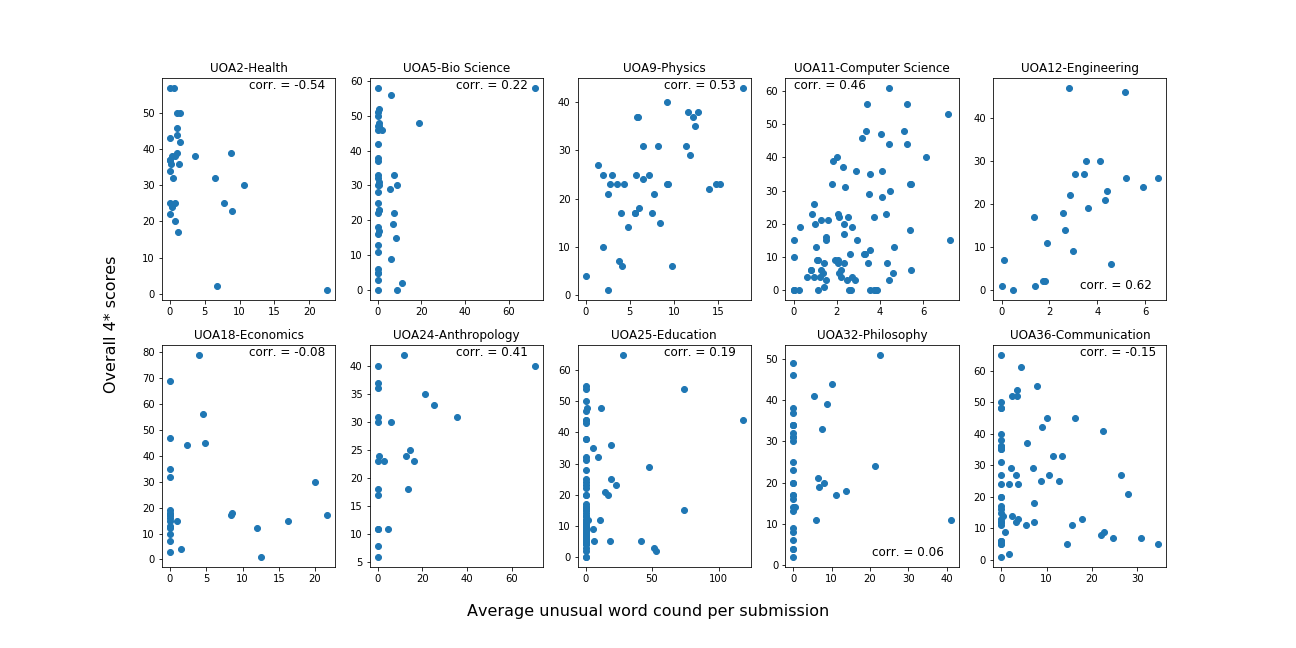
\includegraphics[angle=90,width = 4.2in,keepaspectratio]{overall4star_UWC.png}
  \caption{Average unusual word count per submission vs overall 4* scores plots for every sample UOA.}
  \label{fig:overallUWC}
\end{center}
\end{figure}

\begin{figure}[H]
\begin{center}  \centering
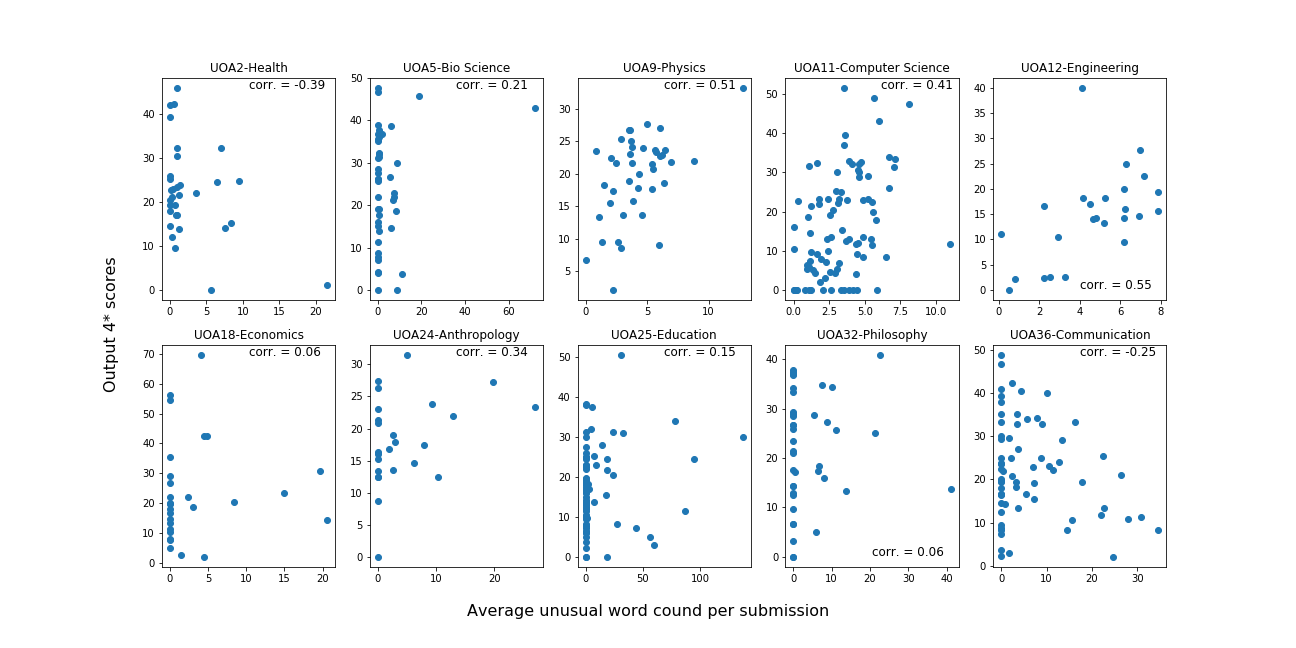
\includegraphics[angle=90,width=4.2in,keepaspectratio]{output4star_UWC.png}
  \caption{Average unusual word count per submission vs output 4* scores plots for every sample UOA.}
  \label{fig:outputUWC}
\end{center}
\end{figure}


\subsubsection{Difference in correlations}

Based on the results above, different levels of correlations were obtained for various UOAs. This section attempts to discuss all the possible reasons behind such difference thus to provide insights into the level of influence additional information has on the scores awarded.\\

\noindent
\emph{Percentage of submissions with additional information}

\noindent
In the first instance, one would suspect the difference in correlations is largely associated with the amount of data available –- the more data there is, the more likely a correlation is going to be found. This could be illustrated in Figure \ref{fig:corr_perc}, which seems to show a trend that Pearson correlation coefficient becomes more positive as more data is given. However, there are two distinctive cases where negative and near-strong negative correlations are seen. \\


\begin{figure}[H]
\begin{center}  \centering
  \includegraphics[width=0.8\textwidth]{Corr_subwithaddinfor.png}
  \caption{Relation between correlation and amount of additional information available.}
  \label{fig:corr_perc}
\end{center}
\end{figure}


\noindent
\emph{Main panels}

\noindent
Table \ref{T:correlation_UWC_4star} shows that the highest positive correlations are mainly found in main panel B, while negative correlations are found in panels A and D respectively. This reflects on the fact that the UOAs in panel B generally provide the largest amount data in the form of additional information, while panel A being the second largest. Strong correlations (both positive and negative) are found in these panels. 




\section{Discussions}
\subsection{Feature 1 - Unusual words in ``Additional Information'' Text}

\subsubsection{Correlations and amount of data available}

In general, the more data available, the stronger the correlation is between unusual word count and 4* scores.

\subsubsection{Negative correlations}

Since 2 out of 10 chosen UOAs are showing negative correlations, it is therefore hard to conclude that unusual word count correlates positively with 4* scores. Further clarification should be made by considering more UOAs. However, given the chosen sample UOAs for this project, it is suggested to look at the main panels in which a UOA belongs on efforts to identify any pattern that gives rise to different directions of correlations.

\subsubsection{Correlations and main panels}

The strongest positive correlations were found mainly in panel B, and negative correlations were also possible in panel A and D.

This could be explained by REF submission requirements -– for additional information, panel A emphasizes the contributions of co-authors and co-researchers, panel B focuses on abstract-like description for the actual work, while panels C and D do not have any strict emphasis \citep{REF_addinforsummary}. This casts a doubt on the previous hypothesis whether a more ``well-written'' and descriptive additional information would give rise to a better score in all main panels, given that the additional information in some panels does not summarise the submissions. Thus, this hypothesis could be modified such that more ``well-written'' additional information only contributes positively to 4* scores for UOAs in panel B. Since mainly co-author/co-researcher information is involved in additional information in panel A, it is reasonable to question to what extent this information contributes to the scores. Therefore, more investigations in panel A are required to clarify whether or not the negative correlation is a coincidence.



\section{Future Research Work}

\subsection{More on ``unusual words''}

\subsubsection{UOA sampling}

\noindent
In the current study, UOAs were sampled randomly across all main panels in the aim of obtaining an overview of how academic disciplines differ from one another in terms of how much each feature contribute differently to the scores in various UOAs. More UOAs should be looked into in the future to focus on the characteristics of one or each of the main panels. For instance, more UOAs in panel A should be examined to determine whether the negative correlation seen in UOA2 is an anomaly or a representative of the entire panel.\\

\noindent
\subsubsection{``Powerful words''}

\noindent
In UOAs where positive correlations are found, it is worth extracting the ``unusual words'' that give rise to high TFIDF values. Analysis could be done in identifying the use of any words that are more likely to result in higher 4* scores -- the ``powerful words''.\\

\noindent
\subsubsection{Overall vs output scores}

\noindent
Theoretically, stronger correlations should be seen between unusual word count and output scores since additional information is directly associated with output submissions. However, the correlations for output are usually less than those for overall for every sampled UOA. Given that the actual content of additional information has no relation with impact or environmental case studies, which contribute to the overall scores, the only possible relation would be the writing style. Knowing that text mining played a part in assessing impact case studies, one might be able to guess that writing style does have an effect on the scores, and this effect is greater on overall results than output since overall rating is associated with the assessment of more text materials. However, this needs to be proved through looking into more UOAs and performing analysis on impact and environmental case studies.




\section{Conclusion}

The counting of unusual words in additional information suggests a possibility, when descriptive texts are part of the requirements of output submission, that a piece of better written additional information might lead to higher scores for the submission, or that a department with diverse research interests (thus less repetitive words) is considered better. 




\renewcommand\refname{Bibliography}

\bibliographystyle{plainnat} % or try abbrvnat or unsrtnat
\bibliography{report_bib} % refers to example.bib

\end{document}